\documentclass[tikz]{standalone}
\usepackage{tikz}
\usetikzlibrary{positioning, graphs}
\usetikzlibrary{graphs.standard}
\usetikzlibrary{arrows.meta}
\begin{document}
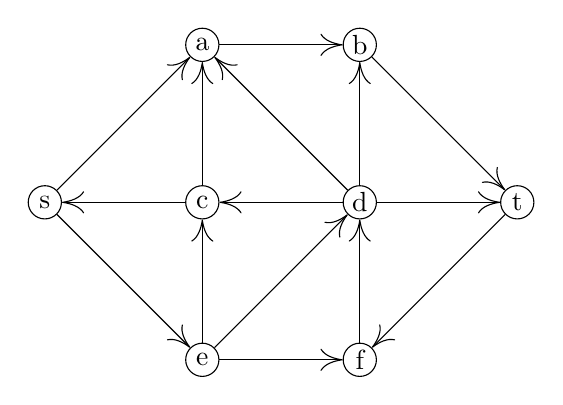
\begin{tikzpicture}
\begin{scope}
		[vertex/.style={draw,circle,inner sep = 0em, minimum size = 1.2em},
		 edgelabel/.style = {fill = white, inner sep = 0.1em, font=\small}]
		\node[vertex] (a) at (0,0) {a};
		\node[vertex] (b) at (2,0) {b};
		\node[vertex] (s) at (-2,-2) {s};
		\node[vertex] (c) at (0,-2) {c};
		\node[vertex] (d) at (2,-2) {d};
		\node[vertex] (t) at (4,-2) {t};
		\node[vertex] (e) at (0,-4) {e};
		\node[vertex] (f) at (2,-4) {f};
		
		\draw[-{>[length=8, width=8]}] (a) to (b);
		\draw[-{>[length=8, width=8]}] (b) to (t);
		\draw[-{>[length=8, width=8]}] (s) to (a);
		\draw[-{>[length=8, width=8]}] (s) to (e);
		\draw[-{>[length=8, width=8]}] (c) to (a);
		\draw[-{>[length=8, width=8]}] (c) to (s);
		\draw[-{>[length=8, width=8]}] (d) to (a);
		\draw[-{>[length=8, width=8]}] (d) to (b);
		\draw[-{>[length=8, width=8]}] (d) to (c);
		\draw[-{>[length=8, width=8]}] (d) to (t);
		\draw[-{>[length=8, width=8]}] (t) to (f);
		\draw[-{>[length=8, width=8]}] (e) to (c);
		\draw[-{>[length=8, width=8]}] (e) to (d);
		\draw[-{>[length=8, width=8]}] (e) to (f);
		\draw[-{>[length=8, width=8]}] (f) to (d);
\end{scope}
\end{tikzpicture}
\end{document}